
% This LaTeX was auto-generated from MATLAB code.
% To make changes, update the MATLAB code and republish this document.

\documentclass{article}
\usepackage{graphicx}
\usepackage{color}

\sloppy
\definecolor{lightgray}{gray}{0.5}
\setlength{\parindent}{0pt}

\begin{document}

    
    
\subsection*{Contents}

\begin{itemize}
\setlength{\itemsep}{-1ex}
   \item Plotting graph of function
   \item Secant Method applied with different intervals.
\end{itemize}
\begin{verbatim}
clear all;
close all;
\end{verbatim}


\subsection*{Plotting graph of function}

\begin{verbatim}
g = @(x) -1.1+0.99403+(1.671*10^-4)*x+(9.7215*10^-8)*x^2-(9.5838*10^-11)*x^3+(1.9520*10^-14)*x^4;
X = -1500:1000; Y = -1500:1000; n = 1;
for x = -1500:1000
Y(n) = g(x);
n = n + 1;
end
plot(X,Y); grid on;
xlabel('Temperature (T)');
ylabel('Zero pressure Specific Heat (c_p)');

fprintf("Considering the interval [-1500, -1000]\n"); SecantMethod(-1500,-1000);
fprintf("Considering the interval [400, 600]\n"); SecantMethod(400,600);
\end{verbatim}

        \color{lightgray} \begin{verbatim}Considering the interval [-1500, -1000]
\end{verbatim} \color{black}
    
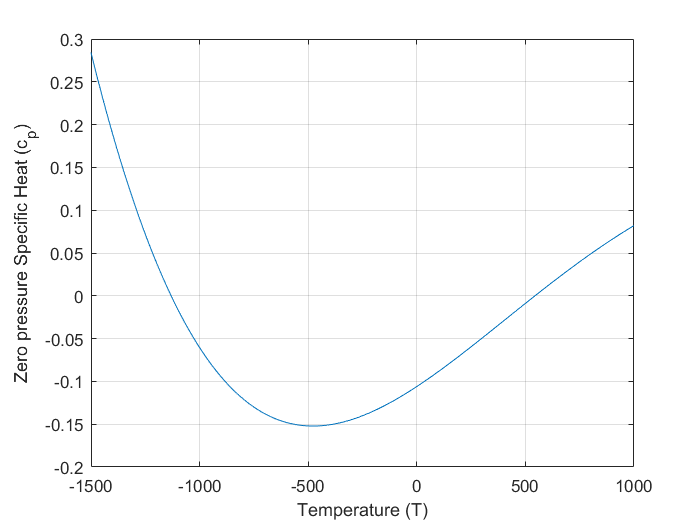
\includegraphics [width=4in]{ques1_secant_01.eps}


\subsection*{Secant Method applied with different intervals.}


\begin{verbatim}x0,x1   initial approximations to location of root\end{verbatim}
    \begin{verbatim}
function y = SecantMethod(x0,x1)
    f = inline('-1.1 + 0.99403 + (1.671*10^-4)*x + (9.7215*10^-8)*x^2 - (9.5838*10^-11)*x^3 + (1.9520*10^-14)*x^4','x');
    TOL=10^(-10); %  absolute error convergence tolerance
    Nmax=100;%   maximum number of iterations to be performed
    flag=0;
    older = x0;   old = x1;
    folder = feval(f,older);
    for i = 2 : Nmax
        fold = feval(f,old);
        dx = fold * ( old - older ) / ( fold - folder );
        new = old - dx;
        fprintf('\t\t %3d \t %.15f \n', i, new )
        if ( abs(dx) < TOL )
            flag=1;
            break
        else
            older = old;
            old = new;
            folder = fold;
        end
    end
    if flag == 0
        disp('Maximum number of iterations exceeded')
    end
end
\end{verbatim}

        \color{lightgray} \begin{verbatim}		   2 	 -1087.706301249115800 
		   3 	 -1138.029509542062000 
		   4 	 -1130.693760893146000 
		   5 	 -1131.025602676162600 
		   6 	 -1131.028101492426900 
		   7 	 -1131.028100596541900 
		   8 	 -1131.028100596544200 
Considering the interval [400, 600]
		   2 	 544.867997840782210 
		   3 	 544.081498954654420 
		   4 	 544.087538233961940 
		   5 	 544.087537655509440 
		   6 	 544.087537655508980 
\end{verbatim} \color{black}
    


\end{document}
    
